\documentclass{standalone}
\usepackage{tikz}
\usepackage{tikz-qtree}
\usetikzlibrary{backgrounds, fit}

\begin{document}
  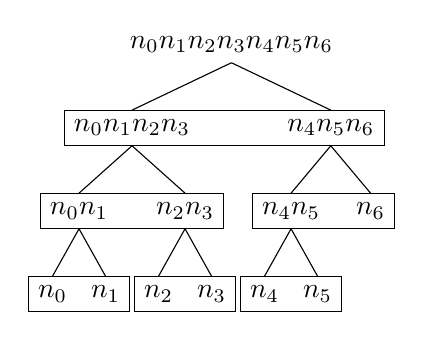
\begin{tikzpicture}
	\Tree [.\node (0123456) {$n_0n_1n_2n_3n_4n_5n_6$};
	  [.\node (0123) {$n_0n_1n_2n_3$};
		[.\node (01) {$n_0n_1$}; 
		  [.\node (0) {$n_0$}; ]
		  [.\node (1) {$n_1$}; ]] 
		[.\node (23) {$n_2n_3$};
		  [.\node (2) {$n_2$}; ]
		  [.\node (3) {$n_3$}; ]]] 
	  [.\node (456) {$n_4n_5n_6$};
		[.\node (45) {$n_4n_5$};
		  [.\node (4) {$n_4$}; ] 
		  [.\node (5) {$n_5$}; ]]
		[.\node (6) {$n_6$}; ]]]

	\begin{pgfonlayer}{background}
	  % \node () [ellipse, draw, fit = (0123456), inner sep = 0pt] {};

	  \node () [rectangle, draw, fit = (0) (1), inner sep = 0pt] {};
	  \node () [rectangle, draw, fit = (2) (3), inner sep = 0pt] {};
	  \node () [rectangle, draw, fit = (4) (5), inner sep = 0pt] {};
	  \node () [rectangle, draw, fit = (01) (23), inner sep = 0pt] {};
	  \node () [rectangle, draw, fit = (45) (6), inner sep = 0pt] {};
	  \node () [rectangle, draw, fit = (0123) (456), inner sep = 0pt] {};
	\end{pgfonlayer}
  \end{tikzpicture}
\end{document}
